\subsection{Application Development }

\subsubsection{Frontend Mobile App Development}


\begin{itemize}
      \item\textbf{Overview}:\\
      Our frontend is designed to provide a user-friendly interface for interacting with the Deepfake Detection App using React Native. It includes features such as user authentication, profile management, and image testing for deepfake detection.

      \item\textbf{Components}:\\
      The frontend consists of several components:

      \begin{itemize}
            \item \textbf{Login Screen}: The login screen serves as the entry point for users to access the application. It presents a clean and intuitive interface where users can input their credentials to authenticate and gain access to their account.

            \item \textbf{Signup Screen}: The signup screen facilitates the registration process through a form where users can input their personal details such as name, email address, and desired password. Upon successful completion of the signup process, users are usually redirected to the login screen to authenticate and access their newly created account.

            \item \textbf{Media Testing Screen}: The media testing screen provides functionality for users to analyze both images and videos for the presence of deepfakes or other forms of manipulation. It offers a straightforward interface for users to upload media files from their device or capture new ones using the device's camera. After uploading a file, the screen initiates a deepfake detection process, using trained modeled to analyze the media and determine its authenticity. The result of the analysis is then displayed to the user, indicating whether the media is likely to be genuine or altered.

            \item \textbf{Profile Screen}: The profile screen provides users with a personalized view of their account information.

            \item \textbf{History Screen}: The history screen allows users to view a chronological record of their past activities within the application. This include a history of logged-in sessions, image testing results. Each entry in the history list includes details such as the date and time of the activity, along with results.
      \end{itemize}

      \item \textbf{Styling}:\\
            The frontend of our application is styled to ensure a seamless user experience, blending custom-styled components with predefined elements from React Native. Custom-styled components are utilized to maintain a cohesive visual identity and streamline the design process, promoting consistency and efficiency.

            \item\textbf{Navigation}:\\
            We have implemented navigation between screens using the React Navigation library. This allows users to navigate seamlessly between different sections of the app.
\end{itemize}

\subsubsection{Backend API Development}

We have used FastAPI to build backend API, providing robust and efficient routing for handling requests and deploying machine learning models trained with Keras for deepfake detection.

\begin{itemize}
      \item \textbf{Overview}:\\
            The backend API serves as the foundation for our Deepfake Detection App, handling various endpoints for user authentication, media testing, and model deployment. It integrates seamlessly with the frontend to provide a cohesive user experience.

      \item \textbf{Endpoints}:\\
            The backend API consists of the following endpoints:

            \begin{itemize}

                  \item \textbf{Authentication Endpoint}\\
                        The authentication endpoint provides a secure mechanism for users to log in and access their accounts. Upon receiving login credentials, the endpoint verifies the provided username and password by comparing them with the hashed credentials stored in the database. To enhance security, the passwords are hashed using the bcrypt hashing algorithm before being stored in the database. If the credentials match, the endpoint generates a JSON Web Token (JWT) containing user information and a unique identifier, which is signed using a secret key. This token is then returned to the client and can be used for subsequent authorized access to protected resources without the need to repeatedly provide credentials.

                        \begin{figure}[htbp]
                              \centering
                              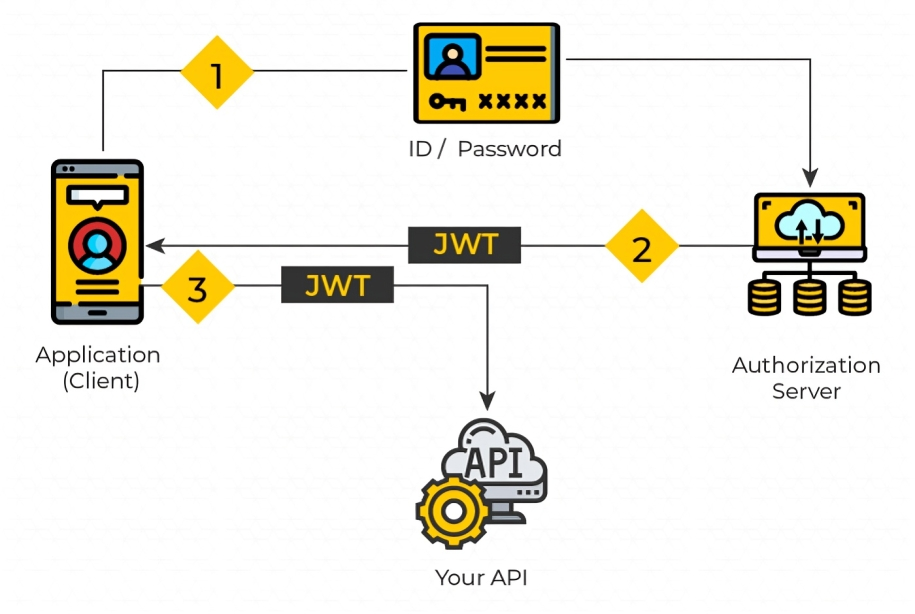
\includegraphics[width=5in]{img/JSON-Web-Tokens-01.png}
                              \caption{JWT Workflow}
                        \end{figure}

                  \item \textbf{Signup Endpoint}:\\
                        The signup endpoint facilitates user registration by processing signup requests and creating new user accounts in the database. The password is securely hashed using the bcrypt algorithm before being stored in the database to protect user privacy. After successful validation and hashing, the endpoint creates a new user account with the provided details and assigns a unique identifier.

                        \begin{figure}[htbp]
                              \centering
                              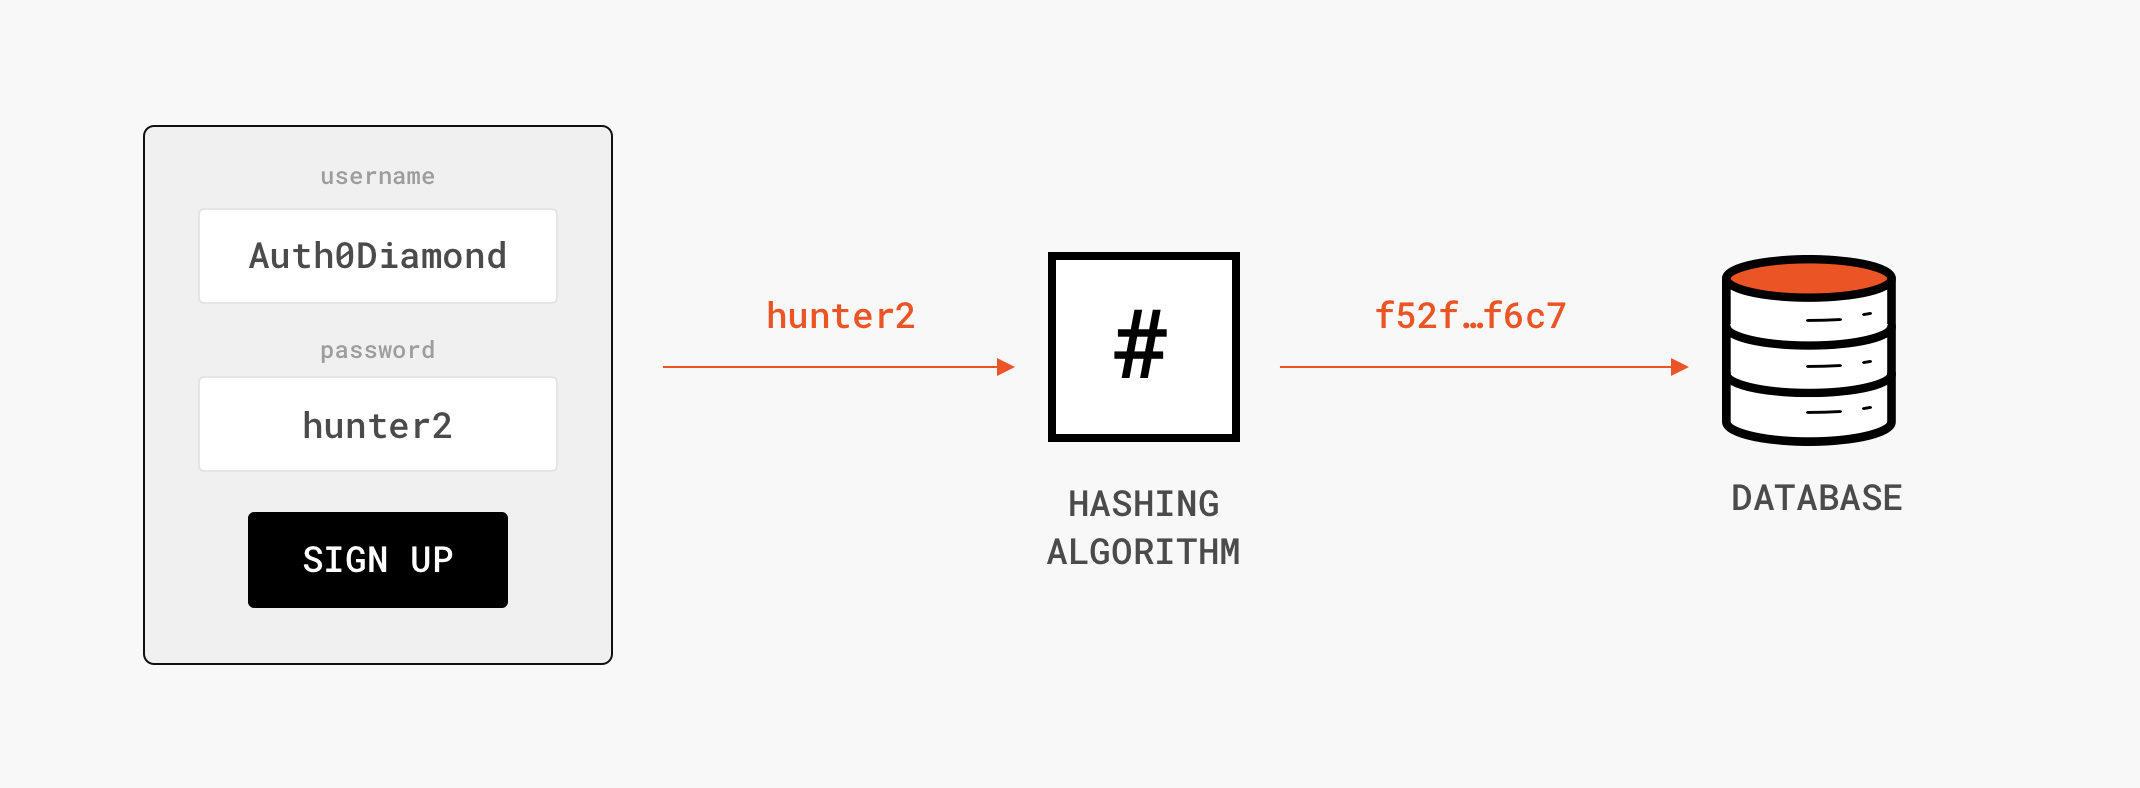
\includegraphics[width=5in]{img/example-of-hashing-during-signup.png}
                              \caption{Hashing}
                        \end{figure}
                  \item \textbf{Media Testing Endpoint}:\\
                        This endpoint is responsible for analyzing images and videos uploaded by users to detect the presence of deepfakes. It utilizes machine learning models deployed with Keras to perform deepfake detection and returns the analysis results to the frontend for display.

                  \item \textbf{Profile Endpoint}:\\
                        The profile endpoint handles requests related to user profiles, allowing users to view their account information.

                  \item \textbf{History Endpoint}: The history endpoint manages user activity logs, maintaining a record of past interactions within the application. It stores information such as login sessions, media testing results, and other relevant data for reference and analysis.
            \end{itemize}

      \item \textbf{Routing and Middleware}:\\
            FastAPI's routing system facilitates the organization and management of various endpoints within our backend application. Through intuitive decorators and path operations, we define the routes that handle incoming HTTP requests and specify the corresponding logic to execute for each request type (GET, POST, PUT, DELETE, etc.).

            Additionally, middleware functions play a crucial role in enhancing the capabilities and security of our backend infrastructure. These middleware components intercept incoming requests and responses, allowing us to implement cross-cutting concerns such as authentication, logging, request validation, and error handling.

            \begin{figure}[htbp]
                  \centering
                  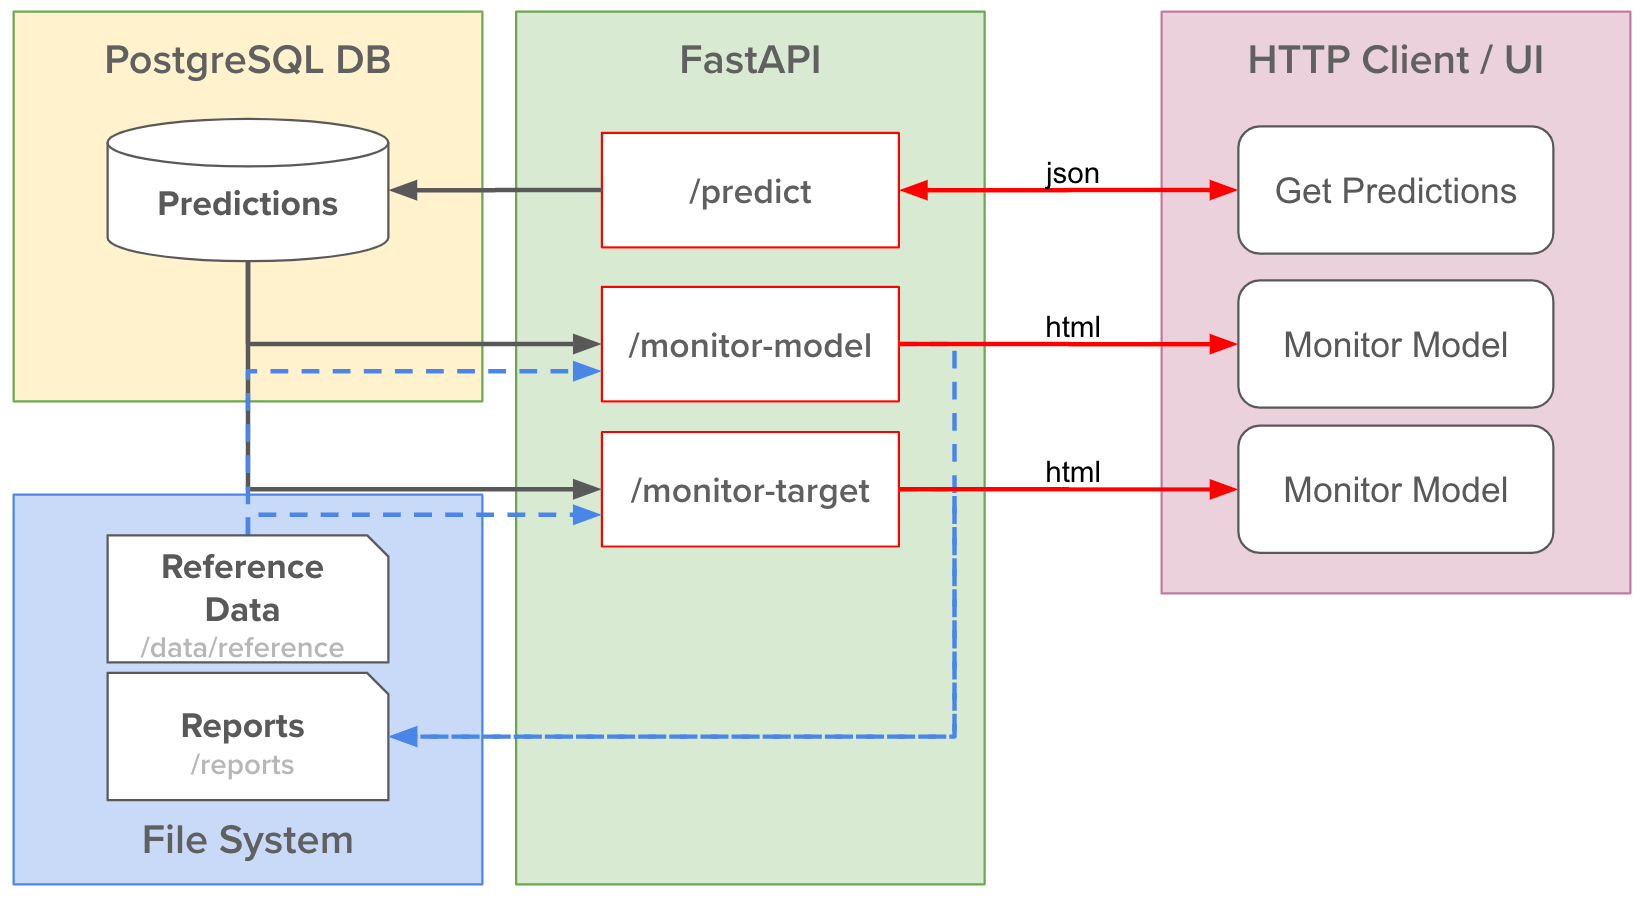
\includegraphics[width=6in]{img/image_2024-02-23_19-12-39.png}
                  \caption{System Workflow Architecture}
            \end{figure}

      \item \textbf{Model Deployment}:\\
            Our backend API integrates machine learning models trained with Keras for deepfake detection. These models are deployed as endpoints within the API, allowing them to process incoming media files and generate predictions on-the-fly. Model deployment is handled efficiently to ensure optimal performance and scalability.

\end{itemize}


\newpage